\chapter{State of the Art}
\label{sec:stateOfTheArt}

schauen dass Sate of the art ca 25 bis 30 seiten hat

\section{Different solutions approaches for rail prediction}

\subsection{Was es alles gibt (1 bis 2 Seiten max)}

\begin{itemize}
    \item Image Classification
    \item Object Detection
    \item Semantic Segmentation (detection und keine direction prediction) hat normalerweise probleme wenn mehrere rails in der scene sind --> weichen schwer trennbar weil der pixelhaufen dazwischen irgendwas ist
    \item Instance Segmentation
    \item panoptic Segmentation
    \item line detection (detection und keine direction prediction) anzahl der rails in einer scene ist das problem
\end{itemize}

was ist das? \\
.\\
Einen absatz mit: \\
im gleichen abschitt aber interesant (für track prediction) sind nur: \\
object detection --> erkennen von switches \\
semantic segmentation \\
lane detection \\
einen kleinen absatz dazu dass object detection mit semantic segmentation verbunden werden kann. (erster ansatz) oder generell dass diese information intressant ist
.\\
Für die nächstem kapitel:\\
was gibt es?\\
was gibt es in der rail domaine?\\

\subsection{Real-time Object detection (2 Seiten)}

\begin{itemize}
    \item Yolov9
    \item Yolov7
    \item ...
\end{itemize}

\subsection{Rail Segmentation oder Semantic Segmentation (2 bis 3 Seiten)}

\begin{itemize}
    \item DeepLab V3+
    \item AdapNet++
    \item ...
\end{itemize}

\subsection{Line detection algorithms (2 bis 3 Seiten)}

Rail Detection: An Efficient Row-based Network and A New Benchmark --> hat auch Lane Detection \& Railroad Detection

\subsection{Backbone architectures 2 Seiten}

\begin{itemize}
    \item EfficientNet 1/2 Seite
    \item ResNet 1/2 Seite
    \item MobileNet 1/2 Seite
    \item DenseNet 1/2 Seite
\end{itemize}

\subsection{mögliches Baseline Paper vielleicht (wenn die Aufteilung geändert werden muss)}

\subsection{verwendetes Baseline Paper vielleicht (wenn die Aufteilung geändert werden muss)}

\subsection{Temporal Models (2 Seiten)}

\begin{itemize}
    \item LSTM -> 1 Seite
    \item GRU -> 1 Seite
    \item ...
\end{itemize}


%%%%%%%%%%%%%%%%%%%%% Datasets %%%%%%%%%%%%%%%%%%%%%

\clearpage                                                       % Beginne neue Seite
\section{Datasets}
\label{sec:datasets}

Datasets are essential for the development of autonomous driving systems, particularly for training and testing algorithms or neural networks.
Typically, raw sensor data is collected from real-world driving scenarios, providing a realistic environment that reflects potential situations the system may encounter in future applications.
This allows for more accurate modeling and evaluation of the system's performance under real conditions.
A common approach to solving problems in autonomous driving systems is using vision-based machine learning algorithms ~\cite[S.~1221]{railsem19dataset}.
These applications typically rely on camera-based data to address various challenges ~\cite[S.~1221]{railsem19dataset}.

Since, autonomous vehicles are increasingly considered a groundbreaking technology of the future \cite{FraunhoferInstituteforCognitiveSystemsIKS} a lot of work is put in the development of such systems.
However often the main focus of this quickly evolving field is on road vehicles, like cars or trucks.
Therefore, most publicly available datasets focus on this application and primarily reflect scenarios in road traffic \cite[S.~1221]{railsem19dataset}.

\subsubsection{Classification Datasets}

There are a couple of public datasets for different \ac{CV} applications. The data of the following datasets are especially gathered for classification tasks.

% ---------------------------------------- Table: Datasets for Classification ----------------------------------------
\begin{table}[H]
\centering
\caption{Datasets for Classification}\label{tab_datsets_classification}
\begin{tabular}{| p{0.3\linewidth} | p{0.3\linewidth} | p{0.3\linewidth} |}\hline
Dataset & Labels & Number of relevant images\\\hline
CIFAR 100 & trains & 600\\\hline
PASCAL VOC2012 & trains & 544\\\hline
Microsoft COCO & trains & 3745\\\hline
1000 ImageNet & \begin{tabular}[c]{@{}l@{}}electric\_locomotive, \\ steam\_locomotive, \\ bullet\_train\end{tabular} & 6722\\\hline
Open Images Dataset V4 & train & 9284\\\hline
\end{tabular}
\end{table}
% --------------------------------------------------------------------------------------------------------------------


\textit{CIFAR 100} dataset \cite{cifar100} consists of small images with pixel size 32x32. This dataset includes 600 images with the label \textit{trains}.
In \textit{PASCAL VOC2012} \cite{pascal2015} there are 544 images labeled \textit{trains}.
\textit{Microsoft COCO} \cite{Lin2014MicrosoftCC} has 3745 images with the class \textit{trains}.
Additionally, there are classes like \textit{traffic lights} and \textit{stop sign}, however theses are not useful to the task of this work because they are from the street domain and not the rail domain.
\textit{1000 ImageNet} \cite{ImageNet2015} includes labels like \textit{electric\_locomotive} (4330 images), \textit{steam\_locomotive} (1187 images) and \textit{bullet\_train} (1205 images).
\textit{Open Images Dataset V4} \cite{openImagesV42018} consists of more than 9.2 million images, annotated with bounding boxes.
Included are 10506 \textit{train}-labels in 9284 images.
However, there are no other significant labels relevant to the rail domain.
Additionally, the dataset contains labels for toy trains, which could pose potential challenges.

\subsubsection{Semantic Segmentation}

Semantic segmentation labels are often refereed to as dense or pixel-wise annotated data.
These datasets are characterized by the fact that each pixel in their images is assigned to a class.

% ---------------------------------------- Table: Datasets for Semantic Segmentation ----------------------------------------
\begin{table}[H]
\centering
\caption{Datasets for Semantic Segmentation}\label{tab_datasets_semanticSegmentation}
\begin{tabular}{| p{0.3\linewidth} | p{0.3\linewidth} | p{0.3\linewidth} |}\hline
Dataset & Labels & Number of relevant images\\\hline
Cityscapes & rail track, train & 284\\\hline
Mapillary Vistas & \begin{tabular}[c]{@{}l@{}}construction-flat-rail-track, \\ object-vehicle-on-rails\end{tabular} & 710\\\hline
COCO-Stuff & platform, railroads, train & 8615\\\hline
KITTI & rail tracks, train & 65\\\hline
\end{tabular}
\end{table}
% ---------------------------------------------------------------------------------------------------------------------------

The \textit{Cityscapes} dataset \cite{cityscapes2016} is commonly used for benchmarks when it comes to road scenes.
It has 35 different labels of which two are \textit{rail track} (131 labels in 117 images) and \textit{train} (194 labels in 167 images).
The \textit{rail track} does not differ between the rails and track bed.
\textit{Mapillary Vistas} \cite{mapillaryVistas2017} also has more labels, but again only two are rail related ones.
\textit{construction-flat-rail-track} is annotated in 710 images and \textit{object-vehicle-on-rails} occurs 272 times.
\textit{COCO-Stuff dataset} \cite{COCO-StuffDataset} includes the same 182 classes like the \textit{Microsoft COCO} \cite{Lin2014MicrosoftCC} but as dense labels.
The rail relevant ones are \textit{railroad} (2839) and \textit{train} (4761).
There is a third rail related label \textit{platform}, however this is a very general label because this can by any plane.
\textit{KITTI} \cite{kittiDataset2018} has the same dense labels like \textit{Cityscapes} \cite{cityscapes2016}.
Likewise, the rail relevant ones are 47 \textit{rail track} and 18 \textit{train} labels.

% Problems with general datsets
These are commonly used datasets in \ac{CV} tasks. However there are there are three main issues when it comes to solving the track prediction use case presented in this work.
Firstly, there is not enough data because the amount of included rail relevant labels is relatively low in each dataset.
Secondly, the labels present are not suitable for training a track prediction algorithm. In this case only the rails, rail tracks or track beds are needed.
Thirdly, the images of the presented datasets are taken out of passengers and pedestrian views. Additionally there are some road views \cite{Hadded.2022}.

% Birds eye views und sign datasets
The datasets mentioned before are very general with a vast amount of different labels.
However there are some datasets specially captured for the rail domain.
As with the other datasets, it is important to consider what specific tasks the datasets are intended to be used for.
There are some datasets captured in the birds eye view to detect damages like cracks in rails \cite{rail5k2021} \cite{ma2024cross} or even some to detect garbage in grooved rails \cite{Huang_2021}. Then there are datasets in ego-perspective of the train driver like \textit{FRSign} \cite{Harb2020FRSignAL} or \textit{GERALD} \cite{leibner2023gerald}, which are created for detecting different traffic lights on French and German railways.

% Überleitung mit Perspective Problem zu ego-perspective datasets
This work deals with Rail Track Prediction, so the system should predict the direction of the track in front of the train. For this particular use case it is most advantages when the dataset is recorded out of the driver cabin in ego-perspective, because it offers a clear sight of the rails in front of the train. Therefore the data has to reflect scenarios, which are comparable. Since the view of the captured images represents a key factor, the before mentioned dataset become unsuitable. An additional reason why these datasets cannot be used for this work is the fact that they are created for different use cases.
Other datasets which deal with the perception in a rail domain environment and are captured in the right perspective are discussed in the following paragraphs.

% ================= Richtige datasets =================

% RailSem19
\subsubsection{RailSem19}
\textit{RailSem19} \cite{railsem19dataset} is the first publicly available dataset fitted for environments in the rail domain. It consists of 8500 annotated images which are gathered from YouTube videos. All of these images are captured in the ego perspective of the train driver, which makes it suitable for the use case of this work. Additionally there are both bounding box labels and dense labels included for object detection and semantic segmentation. The bounding box labels are: \textit{guard-rail; rail; traffic-signal-front; traffic-signal-back; traffic-sign-front; crossing; train; platform; buffer-stop; switch-indicator; switch-static; switch-left; switch-right; switch-unknown}. Important for predicting the direction of the train are the switch labels, because  it gives valuable information. The \textit{switch-unknown} label is used when there is a switch visible but it is unclear in which direction the train would proceed. The presents of this label is mainly due to the high noise levels of the images of YouTube videos.
The dense labels of RailSem19 are: \textit{road; sidewalk; construction; tram-track; fence; pole; traffic-light; traffic-sign; vegetation; terrain; sky; human; rail-track; car; truck; track-bed; on-rails; rail-raised; rail-embedded; void}. In the case of dense labels the labels \textit{tram-track; rail-track; track-bed; on-rails; rail-raised; rail-embedded} are of importance for predicting the direction of trains and trams.
Another advantage is that very diverse environments have been used for this dataset. The creators of \textit{RailSem19} took images from 38 different countries in all four seasons and weather conditions. Additionally, the focus was not only on rails but also on trams, providing a very diverse reflection of rail scenarios and not limiting the use on a specific use case.

\begin{figure}[H]
    \centering
    
    % Erste Reihe
    \begin{subfigure}{0.328\textwidth}
        \includegraphics[width=\linewidth]{PICs/datasets/RailSem19_dataset/RailSem19_Bild1.png}
    \end{subfigure}
    \hfill
    \begin{subfigure}{0.328\textwidth}
        \includegraphics[width=\linewidth]{PICs/datasets/RailSem19_dataset/RailSem19_Bild2.png}
    \end{subfigure}
    \hfill
    \begin{subfigure}{0.328\textwidth}
        \includegraphics[width=\linewidth]{PICs/datasets/RailSem19_dataset/RailSem19_Bild3.png}
    \end{subfigure}

    \vspace{0.1cm} % Größerer Abstand zwischen den Reihen

    % Zweite Reihe
    \begin{subfigure}{0.328\textwidth}
        \includegraphics[width=\linewidth]{PICs/datasets/RailSem19_dataset/RailSem19_Bild1_GT.png}
    \end{subfigure}
    \hfill
    \begin{subfigure}{0.328\textwidth}
        \includegraphics[width=\linewidth]{PICs/datasets/RailSem19_dataset/RailSem19_Bild2_GT.png}
    \end{subfigure}
    \hfill
    \begin{subfigure}{0.328\textwidth}
        \includegraphics[width=\linewidth]{PICs/datasets/RailSem19_dataset/RailSem19_Bild3_GT.png}
    \end{subfigure}

    \caption{RailSem19 dataset examples. First row raw images. Second row dense \ac{GT} \cite{railsem19dataset}.}
    \label{fig:railSem19-images-denseLabels}
\end{figure}

%RailVID
\subsubsection{RailVID}
\label{subsubsec:railVID}
Another dataset that focuses on the detection of rails is the \textit{RailVID} dataset \cite{yuan2022railvid}. The goal of this project is to detect rail tracks and obstacles on the rails, which can lead to possible hazardous situations. With a functioning system, fully automatic train operation is aimed for. The \textit{RailVID} dataset is a collection of 1071 images with the following labels: \textit{background, railway, car, people}. Since, the area of application is on the "Suzhou Rail Transit Line 1" in Jiangsu Province, China all data is captured there. \textit{RailVID} is a collection of infrared data captured with the AT615X infrared thermal instrument from InfiRay. The decision to use infrared data and not RGB images is because it is more robust against challenging imaging conditions, like darkness at night, fog, rain and direct light disturbance.
Since, this dataset only consists of infrared data and in this work \ac{RGB} data should be used, \textit{RailVID} cannot be used fro training. An additional issue is, that the dataset is recorded only on a specific Chinese line. This is advantageous for this particular use case, but it could become an issue if the system were to be deployed elsewhere.

\begin{figure}[H]
    \centering
    \begin{subfigure}{0.24\textwidth}
        \centering
        \includegraphics[width=\linewidth]{PICs/datasets/railVID_dataset/railVID_data.png}
    \end{subfigure}
    \hfill
    \begin{subfigure}{0.24\textwidth}
        \centering
        \includegraphics[width=\linewidth]{PICs/datasets/railVID_dataset/railVID_label.png}
    \end{subfigure}
    \hfill
    \begin{subfigure}{0.24\textwidth}
        \centering
        \includegraphics[width=\linewidth]{PICs/datasets/railVID_dataset/railVID_switch.png}
    \end{subfigure}
    \hfill
    \begin{subfigure}{0.24\textwidth}
        \centering
        \includegraphics[width=\linewidth]{PICs/datasets/railVID_dataset/railVID_switch_label.png}
    \end{subfigure}
    \caption{Example images and \ac{GT} of RailVID dataset \cite{yuan2022railvid}}
    \label{fig:railVID_dataset_images}
\end{figure}

% RailSet
\subsubsection{RailSet}
\cite{railSet2022} and \cite{hadded2022application} presented the \textit{RailSet} dataset,
which is divided into two sub sets: RailSet-Seg for segmentation and RailSet-Ano for anomaly detection \cite{railSet2022}.
Both of them are captured in the ego perspective of the train driver \cite{railSet2022} \cite{hadded2022application}.
The idea is to firstly detect the railways using semantic segmentation and secondly using positional information of the prediction for the creation of the anomaly dataset \cite{railSet2022}.
RailSet-Ano is a collection of 1100 images of railway defects like rail discontinuity and holes in the rail bed.
Some anomalies are taken from a other images and pasted on images of RailSet-Seg and RailSem19 dataset others are generated with a network \cite{railSet2022}.
Since, RailSet-Ano deals with a different use case than the one in this work, this particular data cannot be used.

On the other hand, RailSet-Seg fits the problem. It consists of 6600 images of normal situations.
The images are collected from 23 YouTube videos with a collective duration of 15 hours. It includes two labels: \textit{rail} and \textit{rail-track}.
Besides the use of  RailSet-Seg for the creation of RailSet-Ano, an additional motivation is to include more complex scenes of the rail domain than RailSem19.
That is why the focus of RailSet lies on scenarios with poor weather conditions or lighting conditions.
Furthermore, images are included in which the rails are not visible at all, like in tunnels without lighting or in snowy scenes.
Additionally, it was ensured that the videos were recorded by different cameras and from different mounting positions \cite{railSet2022} \cite{hadded2022application}. 

An advantage of this dataset is that it can be joined with RailSem19, when combining four specific labels.
\textit{trackbed} and \textit{rail-track} from RailSem19 have to be transformed into RailSet's \textit{rail-track} label and \textit{rail-raised} and \textit{rail-embedded} become the \textit{rail} label.
This method leads to more data for the training and validation which could be an advantage.
However, it also shows the disadvantage of this dataset for the specific use case of this work. 
RailSet exclusively addresses railway and not tram scenes \cite{hadded2022application}.
Since, the goal is to target a broad applicability, leaning towards tram scenes this dataset is not used for this work.

% Bild von RailSet
\begin{figure}[H]
    \centering
    \begin{subfigure}{0.3\textwidth}
        \centering
        \includegraphics[width=\linewidth,height=5cm,keepaspectratio]{PICs/datasets/RailSet_dataset/RailSet_image.png}
        \caption{}
        \label{fig:RailSet-Seg_example_image_GT_a}
    \end{subfigure}
    \hspace*{0.02\textwidth} % Abstand manuell steuern
    \begin{subfigure}{0.3\textwidth}
        \centering
        \includegraphics[width=\linewidth,height=5cm,keepaspectratio]{PICs/datasets/RailSet_dataset/RailSet_GT_rails.png}
        \caption{}
        \label{fig:RailSet-Seg_example_image_GT_b}
    \end{subfigure}
    \hspace*{0.02\textwidth} % Abstand manuell steuern
    \begin{subfigure}{0.3\textwidth}
        \centering
        \includegraphics[width=\linewidth,height=5cm,keepaspectratio]{PICs/datasets/RailSet_dataset/RailSet_GT_rails&rail-track.png}
        \caption{}
        \label{fig:RailSet-Seg_example_image_GT_c}
    \end{subfigure}
    \caption{RailSet-Seg example with annotations \cite{railSet2022} \cite{hadded2022application}: \textbf{(a)} raw-image, \textbf{(b)} rail class, \textbf{(c)} rail and rail-track class}
    \label{fig:RailSet-Seg_example_image_GT}
\end{figure}


% RSDS
\subsubsection{RSDS}
The creators of the \ac{RSDS} \cite{railNet2019}, tried to solve the railroad detection problem with a segmentation approach. Because there was no publicly available dataset for this task at the time, they had to construct their own. \ac{RSDS} is captured from the ego perspective of the train driver and is a collection of 3000 images. They used 2500 for training, 200 for validation and 300 for testing. The dataset only includes one \textit{railroad} label. It is described that the labels only incorporate pixels between the two rails and intentionally ignore railway sleepers outside this area. Images are of size 1920 x 1080.
Although it is not mentioned in the paper, it seems as if all images of \ac{RSDS} are captured from a specific rail line in China. Additionally, from the images in the paper alone one can tell that this particular rail line has very distinctive structural characteristics. The colors are bright and it seems like the area between the rails is mostly concrete, which is unusual for most railways. \ref{fig:RSDS_example_image_GT} shows that structures besides the rails are specific too.
One additional detail of this dataset, which can present a disadvantage for this work, is that switches are not addressed.
Since this dataset only covers very specific railroads with unique characteristics and additionally does not address switches or other situations where the track splits, \ac{RSDS} is not further considered for this work.

% Bild von RSDS
\begin{figure}[H]
    \centering
    \begin{subfigure}{0.45\textwidth}
        \includegraphics[width=\linewidth,height=5cm,keepaspectratio]{PICs/datasets/RSDS_dataset/RSDS_image.png}
        \caption{}
        \label{fig:RSDS_example_image_GT_a}
    \end{subfigure}
    \hfill
    \begin{subfigure}{0.45\textwidth}
        \includegraphics[width=\linewidth,height=5cm,keepaspectratio]{PICs/datasets/RSDS_dataset/RSDS_GT.png}
        \caption{}
        \label{fig:RSDS_example_image_GT_b}
    \end{subfigure}
    \caption{\ac{RSDS} example with annotation \cite{railNet2019}: \textbf{(a)} raw-image, \textbf{(b)} ground truth}
    \label{fig:RSDS_example_image_GT}
\end{figure}

% Rail-DB
\subsubsection{Rail-DB}
A very similar dataset is Rail-DB \cite{li2022rail}.
This dataset is a collection of 7432 images, which are taken from 15 videos.
The labels in this dataset are consist of poly lines, which represent all existing rails in an image.
Additionally the the poly lines all have different classes. This way there is not only one rail class, but as many classes as there are rails in one image.
The labeling policy specifies that the central rails are marked with the annotations 1 and 2.
Additional rails are labeled with rising numbers.
Since this dataset includes poly lines and not binary masks, this dataset can be used for training line detection algorithms.
Compared to \ac{RSDS}, this dataset includes not only lines and curves, but also rail switches.
Additionally, the images are taken in various conditions and scenes.
\ref{fig:Rail-DB-dataset_images_annotated} shows example images of Rail-DB's different scenes.
However, it seems that the images again have very specific characteristics like in \ac{RSDS}.
\ref{fig:Rail-DB-dataset_images_annotated} also shows, that all images are captured on a Chinese line.
Even though \cite{li2022rail} presents a very interesting approach for solving the rail detection problem,
because of the before mentioned specific characteristics it is not used for this work. Even the author of \cite{li2022rail} states in the GitHub repository \cite{railNet2022GitHub},
that this project fails to generalize on example videos, where the scene looks different from the one the dataset is captured on.

\begin{figure}[H]
    \centering
    \begin{subfigure}{0.328\textwidth}
        \centering
        \includegraphics[width=\linewidth,height=5cm,keepaspectratio]{PICs/datasets/railDB_dataset/railDB_fog.png}
    \end{subfigure}
    %\hspace*{0.02\textwidth} % Abstand manuell steuern
    \hfill
    \begin{subfigure}{0.328\textwidth}
        \centering
        \includegraphics[width=\linewidth,height=5cm,keepaspectratio]{PICs/datasets/railDB_dataset/railDB_switch.png}
    \end{subfigure}
    %\hspace*{0.02\textwidth} % Abstand manuell steuern
    \hfill
    \begin{subfigure}{0.328\textwidth}
        \centering
        \includegraphics[width=\linewidth,height=5cm,keepaspectratio]{PICs/datasets/railDB_dataset/railDB_night.png}
    \end{subfigure}
    \caption{Rail-DB \cite{li2022rail} images with annotations in different conditions}
    \label{fig:Rail-DB-dataset_images_annotated}
\end{figure}


% OSDaR23
\subsubsection{OSDaR23}
Another dataset it the OSDaR23 \cite{oSDaR23}.
This dataset is a collection of 21 sequences, which are split into 45 subsequences.
Several sequences are short ones with 10 frames each, some are longer with 40 to 100 frames.
In total there are 1534 labeled scenes in this dataset.
Since, OSDaR23 is captured with 9 cameras (\ac{RGB} and \ac{IR}) in different angles, one lidar and one radar sensor, the total number of frames are 1534 * 11 = 16874.
Additionally, position and acceleration sensors are used.
Because also lidar and radar is used, this dataset offers 3D data as well.
OSDaR23 consists of 20 different labels.
These labels include the rail context, like \textit{track}, \textit{switch} or \textit{train} and the environment, like \textit{person}, \textit{animal}, \textit{bicycle}, \textit{smoke}, \textit{flame} or \textit{crowd}.
The annotations for the environment can be used for safety applications.
For more details please refer to \textit{TABLE V} in \cite{oSDaR23}.
\ref{fig:OSDaR23_captured_data} shows the 11 different frames of each sensor and \ref{fig:OSDaR23_annotated} shows an example of an annotated scene.
As illustrated in \ref{fig:OSDaR23_annotated} the \textit{track} label and the \textit{switch} label only offers positional information about their presents, but do not include any information on the direction of the train.
Furthermore, there is no information that distinguishes the train rails from the adjacent rails.
Therefore OSDaR23 can only be used for the detection of rails, but not the track prediction.
Moreover, the capturing of this dataset only took place on rail roads in Hamburg, Germany.
No tram scenes are included.
Due to the necessity of re-labeling for this work and the fact that only data from Hamburg is offered, OSDaR23 is not used.


% captured data
\begin{figure}[H]
    \centering
    % Erstes Bild
    \begin{subfigure}{\textwidth}
        \centering
        \includegraphics[width=0.5\textwidth]{PICs/datasets/OSDaR23_dataset/camerasetup_high_res_cameras.png}
    \end{subfigure}

    % Zweites Bild
    \begin{subfigure}{\textwidth}
        \centering
        \includegraphics[width=0.5\textwidth]{PICs/datasets/OSDaR23_dataset/camerasetup_low_res_cameras.png}
    \end{subfigure}

    % Drittes Bild
    \begin{subfigure}{\textwidth}
        \centering
        \includegraphics[width=0.5\textwidth]{PICs/datasets/OSDaR23_dataset/camerasetup_IR.png}
    \end{subfigure}

    % Viertes Bild
    \begin{subfigure}{\textwidth}
        \centering
        \includegraphics[width=0.5\textwidth]{PICs/datasets/OSDaR23_dataset/camerasetup_Lidar_Radar.png}
    \end{subfigure}
    
    \caption{OSDaR23 data from all different sensors \cite{oSDaR23}}
    \label{fig:OSDaR23_captured_data}
\end{figure}

% labeled scene
\begin{figure}[H]
    \centering
    % Erste Reihe: Zwei Bilder nebeneinander
    \begin{subfigure}{0.45\textwidth}
        \centering
        \includegraphics[width=\textwidth]{PICs/datasets/OSDaR23_dataset/labeled_image.png}
        \caption{\ac{RGB} center camera}
    \end{subfigure}%
    \hspace{0.05\textwidth}
    \begin{subfigure}{0.45\textwidth}
        \centering
        \includegraphics[width=\textwidth]{PICs/datasets/OSDaR23_dataset/labeled_3D.png}
        \caption{merged lidar point cloud}
    \end{subfigure}

    \vspace{0.5cm} % Abstand zwischen den Reihen

    % Zweite Reihe: Zwei Bilder nebeneinander
    \begin{subfigure}{0.45\textwidth}
        \centering
        \includegraphics[width=\textwidth]{PICs/datasets/OSDaR23_dataset/labeled_IR.png}
        \caption{IR center camera}
    \end{subfigure}%
    \hspace{0.05\textwidth}
    \begin{subfigure}{0.45\textwidth}
        \centering
        \includegraphics[width=\textwidth]{PICs/datasets/OSDaR23_dataset/labeled_Radar.png}
        \caption{Radar (zoomed)}
    \end{subfigure}
    
    \caption{OSDaR23 annotated scene \cite{oSDaR23}}
    \label{fig:OSDaR23_annotated}
\end{figure}



\begin{figure}[H]
    \centering
    % Erste Reihe: Zwei Bilder nebeneinander, feste Breite und Höhe
    \begin{subfigure}{0.45\textwidth}
        \centering
        \includegraphics[width=0.9\textwidth,height=5cm]{PICs/datasets/OSDaR23_dataset/labeled_image.png}
        \caption{Bild 1}
    \end{subfigure}%
    \hspace{0.05\textwidth}
    \begin{subfigure}{0.45\textwidth}
        \centering
        \includegraphics[width=0.9\textwidth,height=5cm]{PICs/datasets/OSDaR23_dataset/labeled_3D.png}
        \caption{Bild 2}
    \end{subfigure}

    \vspace{0.5cm} % Abstand zwischen den Reihen

    % Zweite Reihe: Zwei Bilder nebeneinander, gleiche feste Breite und Höhe
    \begin{subfigure}{0.45\textwidth}
        \centering
        \includegraphics[width=0.9\textwidth,height=5cm]{PICs/datasets/OSDaR23_dataset/labeled_IR.png}
        \caption{Bild 3}
    \end{subfigure}%
    \hspace{0.05\textwidth}
    \begin{subfigure}{0.45\textwidth}
        \centering
        \includegraphics[width=0.9\textwidth,height=5cm]{PICs/datasets/OSDaR23_dataset/labeled_Radar.png}
        \caption{Bild 4}
    \end{subfigure}
    
    \caption{OSDaR23 labels skaliert}
\end{figure}

% TEP-Net annotations
\subsubsection{TEP-Net dataset}
\label{subsubsec:TEP-Net_dataset}

\cite{tepNet2024} presents the \ac{TEP}-Net dataset.
The problem this paper aims to solve is rail track prediction.
This differs from all previously mentioned datasets.
No dataset but \cite{tepNet2024} provides information, which distinguishes possible rails in the image from the one the train actually follows.
Since RailSem19 is the most popular dataset in the rail domain, it is used as initial point.
A total of 7917 images were taken from RailSem19.
The remaining 583 were excluded because they are taken from unusual perspectives or it is unclear which track the train is on or would continue on.
Examples of such images are shown in \ref{tep-net_aussortiert}.
These images are excluded simply by not annotating them.
For annotation a new labeling format is created.
Two classes \textit{rail\_right} and \textit{rail\_left} give information about where the tracks of the train  run.
All other rails which might be in the image are ignored.
These two classes consist of poly lines, which are annotated by the corresponding x and y pixel coordinates of the image.
Only the tracks on which the train is located are labeled.
Even if a switch appears in the image and the train would travel over it, only the tracks in the correct direction are further labeled.
This way, switches are indirectly included in this dataset, providing information on the direction a train would continue, even though there is no explicit label for switches.
The poly lines start from lowest pixel row of the images and extend up to a specific horizon line.
Above this horizon further labeling is not possible.
This may occur for various reasons.
The first reason can be an obstruction of the view by the environment or other trains, as shown in \ref{fig:tep-net-annotated-images}.
Since the images are sourced from YouTube videos, it is also possible that the resolution becomes too low in the distance for separately identifying both rails.
Another reason is when it is not possible to determine the direction in which the track continues based on a switch present in an image.
This can happen due to low resolution or unfortunate camera angles.
These cases may be labeled as \textit{switch-unknown} in the original RailSem19 dataset for example.
Here, the polylines stop before the switch.
The polylines from this annotation can then be converted into several different labels using preprocessing algorithms.
On one hand, they can be directly used as polylines.
On the other hand, they can be transformed into a mask for segmentation tasks by filling in the area between the lines.
A third application would be to convert this mask into a grid for classification tasks.

\begin{figure}[H]
    \centering
    \includegraphics[width=\linewidth]{PICs/datasets/TEP_dataset/TEP-Net dataset bilder aussortiert.png}
    \caption{Examples images from RailSem19, which are not included in the \ac{TEP}-Net dataset due to unclear circumstances about the trains direction. \cite{tepNet2024}}
    \label{tep-net_aussortiert}
\end{figure}


\begin{figure}[H]
    \centering
    
    % Erste Reihe
    \begin{subfigure}{0.328\textwidth}
        \includegraphics[width=\linewidth]{PICs/datasets/TEP_dataset/annotated_rs00007.jpg}
    \end{subfigure}
    \hfill
    \begin{subfigure}{0.328\textwidth}
        \includegraphics[width=\linewidth]{PICs/datasets/TEP_dataset/annotated_rs00107.jpg}
    \end{subfigure}
    \hfill
    \begin{subfigure}{0.328\textwidth}
        \includegraphics[width=\linewidth]{PICs/datasets/TEP_dataset/annotated_rs00244.jpg}
    \end{subfigure}

    \vspace{0.1cm} % Größerer Abstand zwischen den Reihen

    % Zweite Reihe
    \begin{subfigure}{0.328\textwidth}
        \includegraphics[width=\linewidth]{PICs/datasets/TEP_dataset/annotated_rs00284.jpg}
    \end{subfigure}
    \hfill
    \begin{subfigure}{0.328\textwidth}
        \includegraphics[width=\linewidth]{PICs/datasets/TEP_dataset/annotated_rs00256.jpg}
    \end{subfigure}
    \hfill
    \begin{subfigure}{0.328\textwidth}
        \includegraphics[width=\linewidth]{PICs/datasets/TEP_dataset/annotated_rs00198.jpg}
    \end{subfigure}

    \caption{\ac{TEP}-Net dataset example images with annotation \cite{tepNet2024}}
    \label{fig:tep-net-annotated-images}
\end{figure}

\textbf{notes wo alles ist}

\begin{itemize}
    \item Railroad Segmentation Dataset (RSDS) --> in RailNet: A Segmentation Network for Railroad Detection fertig
    \item RailSem19 in RailSem19 fertig
    \item RailVID in RailVID fertig
    \item RailSet in RailSet \& Application of Rail Segmentation in the Monitoring of Autonomous Train’s Frontal Environment fertig
    \item Rail-DB (compared to RSDS) --> Rail Detection: An Efficient Row-based Network and A New Benchmark fertig
    \item OSDaR23 in OSDaR23: Open Sensor Data for Rail 2023 fertig
    \item TEP-net dataset fertig
    \item
    \item RailSet -> Segmentation \& Anomaly detection
    \item Application of Rail Segmentation in the Monitoring of Autonomous Train’s Frontal Environment -> RailSegmentation (only rails and trackbed)
\end{itemize}

%%%%%%%%%%%%%%%%%%%%%%%%%%%%%%%%%%%%%%%%%%%%%%%%%%%%%%%%%%%%%%%%%%


%%%%%%%%%%%%%%%%%%%%% Baseline Paper %%%%%%%%%%%%%%%%%%%%%

\clearpage                                                       % Beginne neue Seite
\section{Baseline Paper}
\label{sec:baselinepaper}

To do justice to the contributions of \cite{tepNet2024}, it is addressed in a separate section highlighting the paper's specific insights and relevance. 
To the best of the author's knowledge, \cite{tepNet2024} is the only paper in the literature, which only filters out the two rails the train continuous on, presenting a solution to the rail track prediction problem.
Contrary to most literature, in which often all rails are detected without any distinction between different rails.
Efforts in rail detecting with the trains path in consideration have been made in \cite{RailraodSemanticPossibleTracks2020} and \cite{TPENet2023}.
However, because of the assumption that switch states cannot be accurately determined all "possible rail tracks" are considered in those two papers, leading to complex post-processing.
In \cite{tepNet2024}, the train's rails are defined as the "ego-path" and others are ignored.
To realize a system with this output \cite{tepNet2024} presents a novel regression-based approach, inspired by autonomous driving applications for road cars.

\vspace{0.5cm}

\noindent The main contributions of this work consist of several aspects.
First, unique annotations are created specifically for this project.
Furthermore, a data augmentation strategy is presented, incorporating two distinct cropping techniques for training and inference.
Additionally, a new Regression-based model architecture is developed, to meet the requirements of the novel problem formulation.
A custom loss function is introduced.
In the next few sections, each of these novelties is described in more detail.

\subsection{Annotations}

Since, only the right and left rail of the trains path are detected the dataset needs to be in a corresponding manner.
Therefore \cite{tepNet2024} works with new annotations tailored to this use case and images from the RailSem19 dataset.
This dataset is in the so-called "ego-view", so the cameras are positioned in the driver's cabin and view the rails in front of the train.
The perspective is similar to what a train conductor sees.
For further details of the dataset utilized in this project, please refer to section \ref{subsubsec:TEP-Net_dataset}.

\subsection{Data augmentation}

\cite{tepNet2024} utilizes two data augmentation strategies, one for training and one for inference.
In the Training along wiht usual methods like image color variations and horizontal flips, a cropping mechanism is implemented, which is dependent on th \ac{GT}.
This allows to only focus on the most relevant part of the image, being the "ego-path".
Since, only such crops are used for training, the use case in inference must reflect something similar.
Therefore an autocrop method is developed, which crops images according to a running average of previous predictions.
Both of those techniques are described in \autoref{sec:dataaugmentation} in more detail.


\subsection{TEP-Net Model}

\cite{tepNet2024} proposed a regression-based approach.
For this a model architecture is introduced, which includes a backbone for feature extraction followed by a predictions head.
The head is constructed out of fully connected layers and forms the output at the end.
The output vector, includes the $x$-values for the left and the right rail on anchor lines and a value for the horizon line.
\autoref{fig:TEP-Net_sota_models} shows the proposed regression model in the middle.
A more detailed describtion is given in \autoref{sec:baselineModel}.

\subsection{Loss function}

One of the main contributions is the loss function.
Tailored to the specific use case it is constructed of two functions.
The first one is the trajectory loss, which is responsible for the horizonal error.
The second one is the y-limit loss, which takes the horizon line into account.
Then the two losses are weighted and addded.
For a detailed describtion, plese refer to \autoref{sec:lossFunction}.

\subsection{Experiments, Results and Comparison other state-of-the-art approaches of TEP-Net}

\cite{tepNet2024} compared its appraoch to promising and common methods in the literature: a segmentation and a classifiaction approach.
To fairly compare the novel regression-based architecture, \cite{tepNet2024} uses the same backbone and replaces the prediction heads, as illustrated in \autoref{fig:TEP-Net_sota_models}.
The segmentation model utilizes a U-Net-like \cite{uNet2015} decoder, which outputs a binary mask with dimensions $1 \times 512 \times 512$.
A binary Dice loss is used for training.
The classification model is inspired by \cite{li2022rail} and follows their settings.
It outputs a $2 \times 64 \times (128 + 1) = 16512$-dimensional vector.
$2$ grids for 2 rails, with a height of $64$ and a width of $128+1$.
The $+1$ is for the background class.
A cross-entropy loss is used to train this model \cite{tepNet2024}.
For experiments, the same dataset is utilized with various preprocessing steps to fit the specific task of the model.

\begin{figure}[H]
    \centering
    \includegraphics[width=\linewidth]{PICs/Baselinepaper/tep-net_sota_models.jpg}
    \caption{The model architecture is designed to enable a fair comparison between the novel regression model proposed in \cite{tepNet2024} and other \ac{SOTA} approaches.
    All models use the same dataset with preprocessing steps to fit annotation to the model task.}
    \label{fig:TEP-Net_sota_models}
\end{figure}

Experiments include trainings with different backbones: ResNet18, 34, 50 and EfficientNet B0, B1, B2, B3.
Results of \cite{tepNet2024} show that the segmentation-based approach is the most accurate when it comes to the \ac{IoU}.
However, the difference in \ac{IoU} performances is within a range of only 1.4 percent.
Classification with ResNet18 performs worst.
While segmenation with EfficientNet-B3 achieves the highest accuracy, it is also the slowest.
In terms of speed the regression-based approach outperforms other models.
Additionally, it proves to be light weight because of lower number in parameters and \ac{MACs}.
These characteristics are of great importance for the rail track prediction application of this work.
For more detailed results, please refer to \cite{tepNet2024}.

\begin{figure}[H]
    \centering
    \includegraphics[width=0.7\linewidth]{PICs/Baselinepaper/comparison_sota_tep-net_modified.jpg}
    \caption{Comparison between classification (CLS), regression (REG) and segmentation (SEG) models with challenging scenes.
    The worst backbone (ResNet18) is used for this figure to clearly show difference in behaviours \cite{tepNet2024}.}
    \label{fig:TEP-Net_sota_comparison}
\end{figure}

Since all three model architectures achieve similar \ac{IoU} scores, \cite{tepNet2024} compares performances on individual challenging scenes.
\autoref{fig:TEP-Net_sota_comparison} visualizes a drop in accuracy when the model becomes unsure.
However, the regression model is the only one which keeps the form of a rail when the track splits and seems to no issues with obstructions.
This is because the concept of distance in the error between prediction and \ac{GT} is only provided in the regression-based model, but missing in segmentation and classification models.
The cross-entropy loss for classification and the dice loss for segmentation both penalize misclassifications but do no account for increasing distance from the \ac{GT}.
These models work with probabilities, which tend towards extrems under certainty.
When uncertain segmenation models move closer to a threshold and classification models show more spread-out probabilities across classes.
The regression appraoch inherently involves continuous values, which assumes averages among uncertain possibilities.
Resulting in a more robust system \cite{tepNet2024}.

\subsection{Limitation}

The main limitation of \cite{tepNet2024} lies in its single-frame-based model architecture.
This model cannot capture temporal context, which becomes problematic when the train encounters a switch.
An example scenario is illustrated in \autoref{fig:limitationSwitch}.
Typically, the model effectively predicts the train's path when approaching switches, with all necessary information contained within the frame.
However, once the train passes over the switch and the start of the switch is no longer visible, the model cannot determine the continuation of the ego path.
Only after a certain duration, does the correct track become identifiable again.

\begin{figure}[H]
    \centering

    % Oberes Grid mit großen Bildern
    \begin{minipage}{0.328\textwidth}
        \includegraphics[width=\textwidth]{PICs/Baselinepaper/limitation_1.png}
    \end{minipage}
    \hfill
    \begin{minipage}{0.328\textwidth}
        \includegraphics[width=\textwidth]{PICs/Baselinepaper/limitation_3.png}
    \end{minipage}
    \hfill
    \begin{minipage}{0.328\textwidth}
        \includegraphics[width=\textwidth]{PICs/Baselinepaper/limitation_5.png}
    \end{minipage}

    \vspace{-0.15cm} % Kleinerer Abstand
    
    % Dritte Reihe nur für die Pfeile (zwischen oberen und unteren Bildern)
    \begin{minipage}{0.16\textwidth}
        \begin{tikzpicture}
            \node[anchor=south] (img) at (0,0) {};
            \draw[->, thick] (1.1,-0.1) -- (1.1,0.1); % Kürzerer Pfeil nach oben für das 1. Bild der unteren Reihe
        \end{tikzpicture}
    \end{minipage}
    \hfill
    \begin{minipage}{0.16\textwidth}
        % Kein Pfeil für dieses Bild
    \end{minipage}
    \hfill
    \begin{minipage}{0.16\textwidth}
        \begin{tikzpicture}
            \node[anchor=south] (img) at (0,0) {};
            \draw[->, thick] (0.5,-0.1) -- (0.5,0.1); % Kürzerer Pfeil nach oben für das 3. Bild der unteren Reihe
        \end{tikzpicture}
    \end{minipage}
    \hfill
    \begin{minipage}{0.16\textwidth}
        % Kein Pfeil für dieses Bild
    \end{minipage}
    \hfill
    \begin{minipage}{0.16\textwidth}
        \begin{tikzpicture}
            \node[anchor=south] (img) at (0,0) {};
            \draw[->, thick] (0.1,-0.1) -- (0.1,0.1); % Kürzerer Pfeil nach oben für das 5. Bild der unteren Reihe
        \end{tikzpicture}
    \end{minipage}
    \hfill
    \begin{minipage}{0.16\textwidth}
        % Kein Pfeil für dieses Bild
    \end{minipage}
    
    % Unteres Grid mit kleineren Bildern
    \begin{minipage}{0.16\textwidth}
        \includegraphics[width=\textwidth]{PICs/Baselinepaper/limitation_1.png}
    \end{minipage}
    \hfill
    \begin{minipage}{0.16\textwidth}
        \includegraphics[width=\textwidth]{PICs/Baselinepaper/limitation_2.png}
    \end{minipage}
    \hfill
    \begin{minipage}{0.16\textwidth}
        \includegraphics[width=\textwidth]{PICs/Baselinepaper/limitation_3.png}
    \end{minipage}
    \hfill
    \begin{minipage}{0.16\textwidth}
        \includegraphics[width=\textwidth]{PICs/Baselinepaper/limitation_4.png}
    \end{minipage}
    \hfill
    \begin{minipage}{0.16\textwidth}
        \includegraphics[width=\textwidth]{PICs/Baselinepaper/limitation_5.png}
    \end{minipage}
    \hfill
    \begin{minipage}{0.16\textwidth}
        \includegraphics[width=\textwidth]{PICs/Baselinepaper/limitation_6.png}
    \end{minipage}

    % Vierte Reihe für die Zeitachse
    \begin{minipage}{1.0\textwidth}
        \centering
        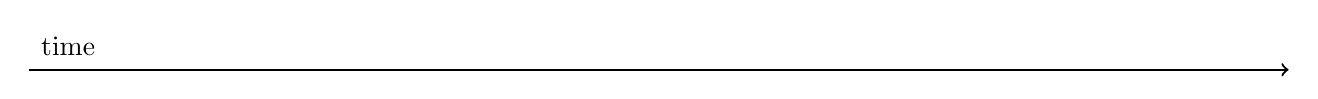
\begin{tikzpicture}
            % Zeit "Time" über dem Pfeil links positionieren
            \node at (-7.5, 0.3) {time}; % Text "Time"
            \draw[->, thick] (-8, 0) -- (8, 0); % Pfeil von ganz links nach ganz rechts
        \end{tikzpicture}
    \end{minipage}

    % Beschriftung unter dem Grid
    \vspace{0.5cm}
    \caption{Limitation of \ac{TEP}-Net \cite{tepNet2024}. The introduced approach is a single-frame-based model. Therefore, no temporal context can be captured, which leads to uncertainty in prediction when driving over a switch.
    All images are from \cite{limitaion_youtube_video}. A YouTube video, which is also used by RailSem19. It is ensured that none of the frames are included in the dataset, creating a fair test scenario.}
    \label{fig:limitationSwitch}
\end{figure}

There are two approaches suggested in \cite{tepNet2024}.
The first one includes integrating a confidence score to tell if the model is in a scenario where it is prone to become unreliable.
The second suggested approach is more complete.
It would encounter the temporal component by implementing a model like a \ac{RNN}, that can capture temporal information.
However, \cite{tepNet2024} states that there is no public temporal dataset available, which fits this task.
To the best of the author knowledge, this statement is correct.
Therefore, a corresponding dataset must also be created, if this approach is pursued.

%%%%%%%%%%%%%%%%%%%%%%%%%%%%%%%%%%%%%%%%%%%%%%%%%%%%%%%%%%%%%%%%%%